\documentclass[10pt]{article}
\usepackage[margin=1in]{geometry}
\usepackage[T1]{fontenc}
\usepackage[utf8]{inputenc}
\usepackage{lmodern}
\usepackage{microtype}
\usepackage{amsmath}
\usepackage{amssymb}
\usepackage{booktabs}
\usepackage{graphicx}
\usepackage{hyperref}
\usepackage{xcolor}

\title{Theory Report: Conditional Audio Autoencoding for UrbanSound8K}
\author{Kirill Shumskiy, Ekaterina Petrova}
\date{\today}

\begin{document}
\maketitle

\noindent Repository: \href{https://github.com/I-y6o-I/s26_genai_project/tree/main}{https://github.com/I-y6o-I/s26\_genai\_project/tree/main}

\section{Task Setup and Reproducibility}
Our goal is class-conditional audio generation on UrbanSound8K using spectrogram-based latent-variable models.
Each input is converted to a log-mel spectrogram with sample rate 22{,}050 Hz, \texttt{n\_mels=128}, \texttt{n\_fft=2048}, and \texttt{hop=512}.
The time axis is padded or cropped to \texttt{spec\_t=176}, then normalized approximately to \([-1,1]\).
This gives a fixed input tensor \(x \in \mathbb{R}^{1 \times 128 \times 176}\) and a class label \(y \in \{0,\dots,9\}\).

The code path is reproducible from the repository:
\texttt{src/train.py} defines training, \texttt{src/eval.py} defines evaluation and qualitative export, and run artifacts are written under \texttt{experiments/cae/} and \texttt{experiments/cvae/}.
Each run stores a checkpoint, config, history, and metrics JSON/CSV files.
The current sweeps use a fixed validation ratio of \(0.1\), fixed seed \(42\), AdamW, cosine learning-rate decay, gradient clipping, checkpointing, and early stopping.

\begin{figure}[h]
\centering
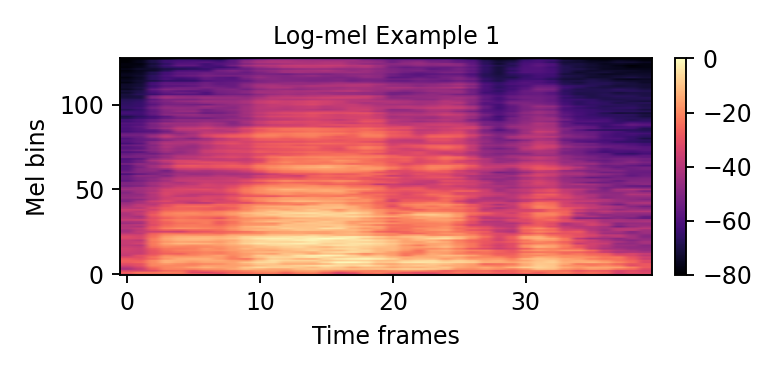
\includegraphics[width=0.47\linewidth]{figures/spec_example_1.png}
\hfill
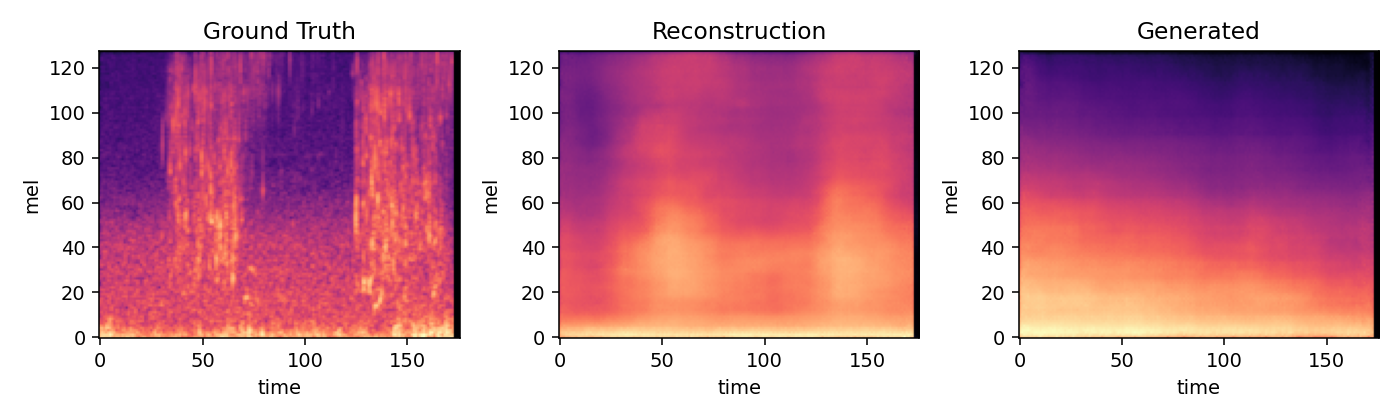
\includegraphics[width=0.47\linewidth]{../experiments/cvae/cvae_nb_005_20260319_023146_lat64_lr0.0003_bs64_st176_nm128_fft2048_hop512_bkl0.001/qualitative_classpost_ns050/sample_000_class_3/spectrograms.png}
\caption{Left: preprocessed log-mel input. Right: qualitative example from the current best cVAE run, showing ground truth, reconstruction, and class-conditional generation.}
\end{figure}

\section{Model Definition}
We implemented two closely related conditional models:

\paragraph{Conditional Autoencoder (AE).}
The encoder \(E_\phi(x, y)\) is a residual convolutional network with four downsampling blocks.
Class information is injected through a learned label embedding, concatenated with the flattened convolutional representation.
The decoder \(D_\theta(z, y)\) mirrors the encoder with transposed-convolution residual blocks and reconstructs the spectrogram.

\paragraph{Conditional Variational Autoencoder (cVAE).}
The cVAE uses the same conditional backbone but replaces the deterministic encoder output with Gaussian parameters
\[
q_\phi(z \mid x, y) = \mathcal{N}\bigl(\mu_\phi(x,y), \operatorname{diag}(\sigma_\phi^2(x,y))\bigr).
\]
Sampling uses the standard reparameterization trick
\[
z = \mu_\phi(x,y) + \sigma_\phi(x,y)\odot \varepsilon,\qquad \varepsilon \sim \mathcal{N}(0, I).
\]
The decoder again predicts a spectrogram \(\hat{x} = D_\theta(z, y)\).

Both models are intentionally lightweight and operate in spectrogram space rather than waveform space.
This keeps training simple and makes failure analysis easier, but it also means waveform quality depends on Griffin--Lim inversion during evaluation.

\section{Training Objective and Optimization}
For the AE, the objective is pure spectrogram reconstruction:
\[
\mathcal{L}_{\text{AE}}(x,\hat{x}) = \|x - \hat{x}\|_1.
\]

For the cVAE, we optimize
\[
\mathcal{L}_{\text{VAE}}(x,\hat{x},\mu,\log \sigma^2)
= \|x - \hat{x}\|_1
+ \beta \, D_{\mathrm{KL}}\bigl(q_\phi(z \mid x,y)\,\|\,\mathcal{N}(0,I)\bigr),
\]
where
\[
D_{\mathrm{KL}} = -\frac{1}{2}\sum_i \left(1 + \log \sigma_i^2 - \mu_i^2 - \sigma_i^2\right).
\]

Optimization details are the same across the main sweeps unless explicitly changed:
\begin{itemize}
\item optimizer: AdamW,
\item learning rate: \(10^{-4}\) or \(3\cdot 10^{-4}\),
\item batch size: \(64\),
\item gradient clipping: \(1.0\),
\item scheduler: cosine annealing,
\item early stopping on validation loss,
\item checkpoint selection by best validation objective.
\end{itemize}

The baseline AE was trained first to verify the code path and objective implementation.
The cVAE was then introduced because the AE has no reason to learn a sampleable latent prior.
This model change is the main theory-driven intervention in the project so far.

\begin{figure}[h]
\centering
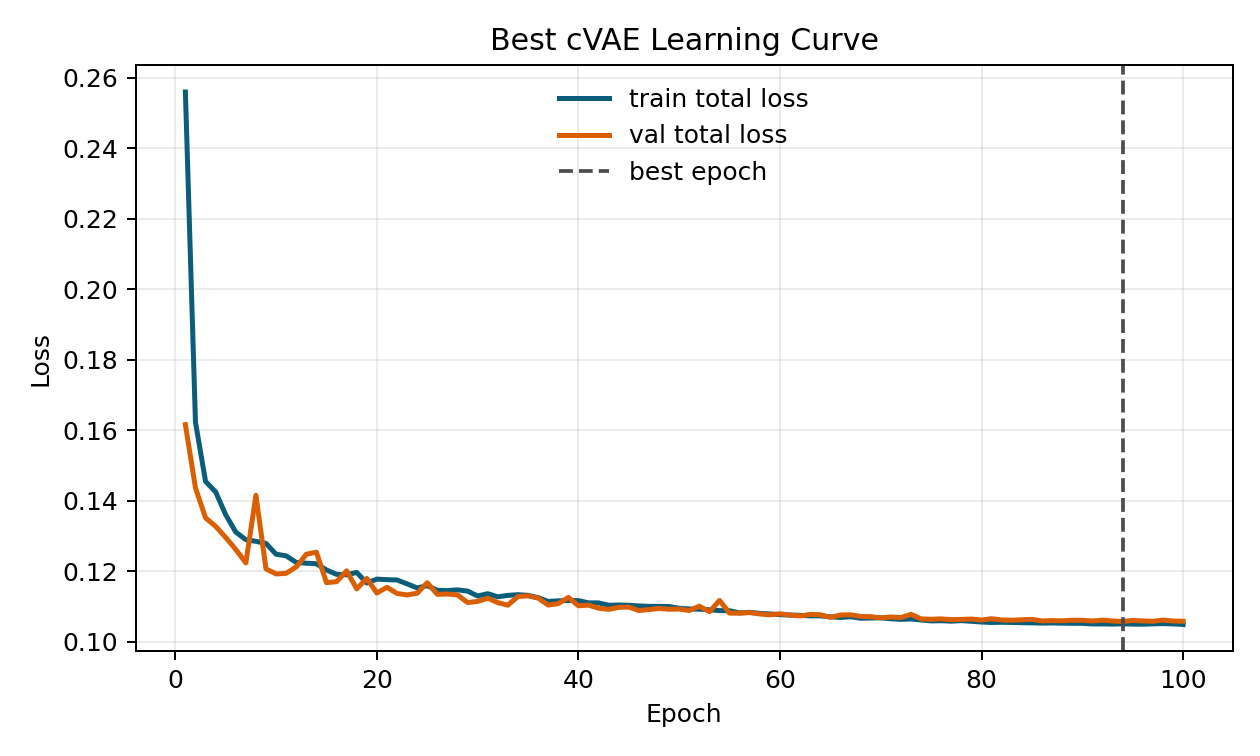
\includegraphics[width=0.70\linewidth]{figures/cvae_learning_curve.png}
\caption{Learning curve of the current best cVAE run (\texttt{cvae\_nb\_005}). The model keeps improving well beyond the first epochs, unlike the earlier AE runs that often saturated very early.}
\end{figure}

\section{Evaluation Protocol}
We evaluate both reconstruction and generation.
Reconstruction metrics are log-mel L1, multi-resolution STFT loss, and SI-SDR after Griffin--Lim inversion.
Generation metrics are latent-space FAD and embedding diversity, computed by using the model encoder as a deterministic feature extractor.
Qualitative outputs are also exported as \texttt{spectrograms.png}, \texttt{gt.wav}, \texttt{recon.wav}, and \texttt{gen.wav}.

This protocol is useful for fast iteration, but it has a caveat: FAD and diversity are measured in a model-dependent embedding space, so comparisons are most reliable within one model family.
Negative SI-SDR values are also expected here, because the model is not waveform-supervised and Griffin--Lim inversion is lossy.

\section{Results and Controlled Comparisons}
\subsection{Controlled Comparison 1: AE vs cVAE}
The clearest controlled comparison is the best AE run versus the best cVAE run under the same dataset and spectrogram setup.
Table~\ref{tab:ae_vs_cvae} shows that the cVAE improves both reconstruction and generation quality.
The improvement in FAD is especially important: the AE is a weak generator, while the cVAE at least learns a usable sampling space.

\begin{table}[h]
\centering
\caption{Best AE vs best cVAE.}
\label{tab:ae_vs_cvae}
\begin{tabular}{lccccc}
\toprule
Model & Best val & Log-mel L1 & MR-STFT & FAD & Fake div. \\
\midrule
AE (\texttt{lat256, lr=3e-4}) & 0.1081 & 0.1081 & 2.0958 & 41224.8 & 0.0914 \\
cVAE (\texttt{lat64, lr=3e-4, \(\beta=10^{-3}\)}) & \textbf{0.1058} & \textbf{0.0918} & \textbf{1.8971} & \textbf{3.0198} & \textbf{0.1851} \\
\bottomrule
\end{tabular}
\end{table}

The AE reproduces training inputs reasonably well but completely fails to define a generation prior.
In contrast, the cVAE keeps reconstruction strong while reducing FAD by several orders of magnitude.
This supports the correctness of the cVAE objective and the implementation of reparameterization and KL regularization.

\subsection{Controlled Comparison 2: cVAE Hyperparameters}
The cVAE sweep gives two useful controlled comparisons.
First, lowering the learning rate from \(3\cdot 10^{-4}\) to \(10^{-4}\) consistently hurts both reconstruction and FAD at the same \(\beta\).
Second, increasing latent dimensionality from 64 to 128 does not improve results enough to justify the larger model.

\begin{table}[h]
\centering
\caption{Selected cVAE ablations from the six-run sweep.}
\label{tab:cvae_ablation}
\begin{tabular}{lcccc}
\toprule
Setting & Best val & Log-mel L1 & FAD & Div. ratio \\
\midrule
\texttt{lat64, lr=3e-4, \(\beta=10^{-3}\)} & \textbf{0.1058} & \textbf{0.0918} & \textbf{3.0198} & \textbf{0.5711} \\
\texttt{lat128, lr=3e-4, \(\beta=10^{-3}\)} & 0.1060 & 0.0925 & 3.3379 & 0.5311 \\
\texttt{lat64, lr=1e-4, \(\beta=10^{-3}\)} & 0.1095 & 0.0957 & 3.5746 & 0.5312 \\
\texttt{lat256, lr=1e-4, \(\beta=5\cdot 10^{-3}\)} & 0.1413 & 0.1209 & 0.9859 & 0.5658 \\
\bottomrule
\end{tabular}
\end{table}

The last row is interesting: stronger KL regularization produced the numerically best FAD, but reconstruction degraded sharply.
This means the model was pushed toward a more regular latent prior, yet the decoded samples became too weak as reconstructions.
So far, the best trade-off is still the smaller cVAE with \(\beta=10^{-3}\), latent size 64, and learning rate \(3\cdot 10^{-4}\).

\subsection{Controlled Comparison 3: Sampling Ablation Beyond the Sweep}
We also ran a focused ablation on the best cVAE checkpoint, keeping the model fixed and changing only the sampling rule at inference time.
This isolates a question that the original sweep did not answer: is the standard normal prior already good enough, or does generation improve if we sample from a class-conditional empirical posterior estimated from validation latents?

We compared two modes at the same \texttt{noise\_std=0.5} over five random seeds:
\begin{itemize}
\item \textbf{Prior}: \(z \sim \mathcal{N}(0, I)\),
\item \textbf{Class posterior}: \(z \sim \mathcal{N}(\mu_c, \Sigma_c)\), where \(\mu_c\) and \(\Sigma_c\) are estimated from latent codes of class \(c\).
\end{itemize}

The result is a genuine trade-off.
Class-posterior sampling improves mean FAD from \(2.255 \pm 0.038\) to \(\mathbf{2.202 \pm 0.055}\), but decreases the fake/real diversity ratio from \(0.699 \pm 0.003\) to \(0.676 \pm 0.007\).
So the empirical class-conditional latent statistics help the generated distribution move closer to real data in embedding space, but they also make samples slightly less diverse.
This is useful failure analysis: the bottleneck is no longer only model capacity, but also prior mismatch versus diversity preservation.

\begin{figure}[h]
\centering
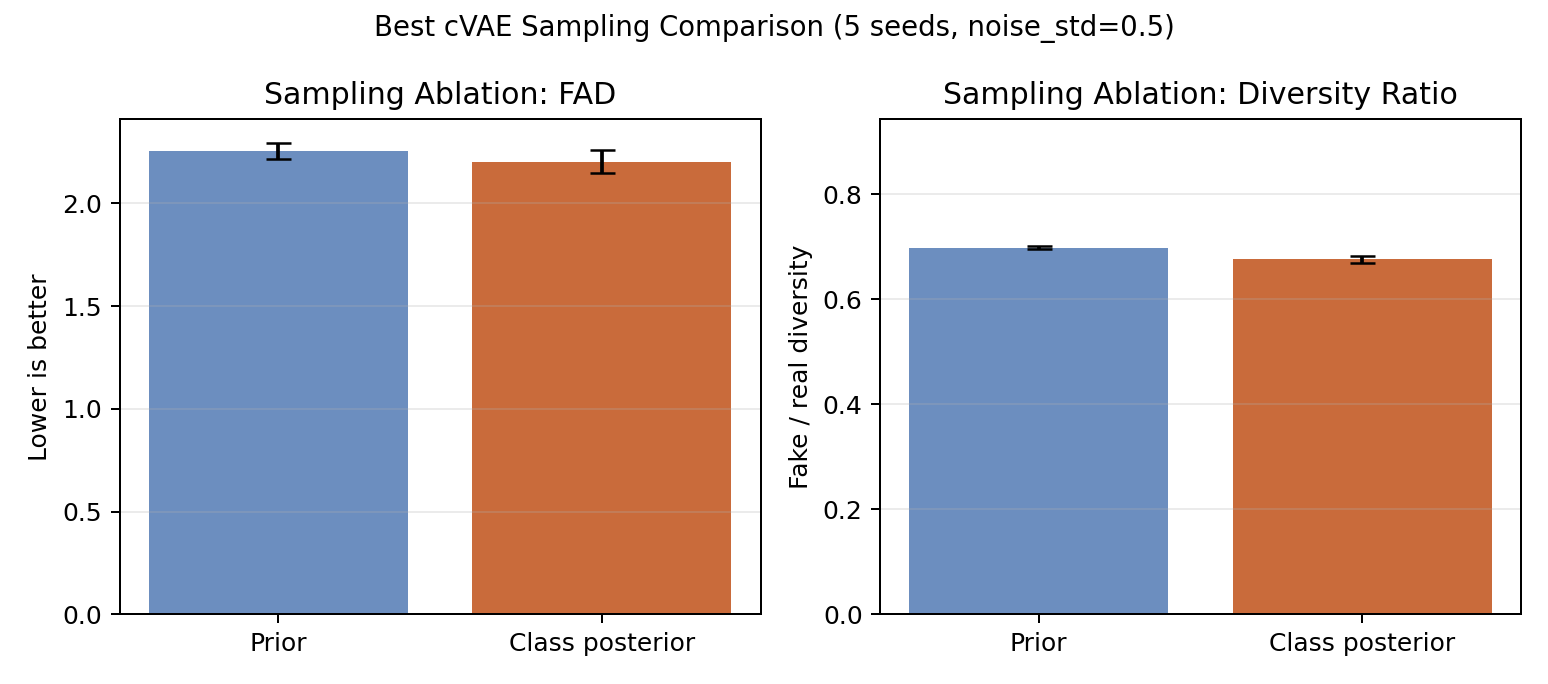
\includegraphics[width=0.82\linewidth]{figures/cvae_sampling_ablation.png}
\caption{Sampling ablation on the best cVAE checkpoint over five random seeds. Class-posterior sampling improves FAD, while prior sampling retains slightly higher diversity.}
\end{figure}

\subsection{Reproducibility Evidence}
We also have a small reproducibility signal inside the cVAE sweep.
Runs \texttt{cvae\_nb\_001} and \texttt{cvae\_nb\_005} share the same hyperparameters and end up in the same quality range:
best validation loss \(0.1066\) vs \(0.1058\), log-mel L1 \(0.0931\) vs \(0.0918\), and FAD \(3.36\) vs \(3.02\).
This is not a full multi-seed study, but it suggests the pipeline is stable enough to continue systematic work.

\section{Failure Analysis and Planned Improvements}
The main failure mode is still under-dispersed generation.
Even the best cVAE produces fake diversity only about \(57\%\) of real embedding diversity.
Qualitatively, reconstructions are often recognizable, but unconditional samples can sound over-smoothed or class-generic.

We identified three likely causes:
\begin{enumerate}
\item spectrogram-only supervision encourages averaged reconstructions;
\item a fixed standard-normal prior is still mismatched to the empirical latent distribution;
\item Griffin--Lim is a weak waveform decoder and amplifies artifacts.
\end{enumerate}

To address this, we added latent-statistics-based sampling for the cVAE, so generation can use aggregate or class-conditional posterior statistics instead of only \(z \sim \mathcal{N}(0, I)\).
The ablation above shows that this already improves FAD for the current best checkpoint, but it is still not a substitute for a better training objective.

The next planned improvements are:
\begin{itemize}
\item KL warmup or free bits, to avoid the current reconstruction--regularization trade-off;
\item repeated-seed experiments for the best cVAE configuration;
\item external audio embeddings for more trustworthy FAD-style evaluation;
\item a stronger waveform decoder or vocoder for qualitative audio;
\item potentially a more expressive generator (e.g.\ VQ-VAE or diffusion-based decoder) if the cVAE ceiling remains low.
\end{itemize}

\section*{Conclusion}
The project has moved from a correct but non-generative conditional AE baseline to a cVAE that is both reproducible and measurably better as a generator.
The objective and implementation appear correct: the sanity checks pass, the pipeline is runnable end-to-end, and the cVAE improves all core metrics over the AE.
However, the current model is still only a moderate generator, not a final-quality one.
The most defensible conclusion is that latent regularization helps substantially, but better prior matching and better audio decoding are still the next necessary steps.

\end{document}
